% --- Pruning ---
\begin{frame}[plain]
  \centering
  \vfill
  {\LARGE\bfseries Pruning}
  \vfill
\end{frame}

\begin{frame}{Compression Technique: Pruning}
  \begin{itemize}\itemsep0.3em
    \item[\textcolor{red}{$\blacktriangleright$}] Trained networks are heavily over-parameterised: many weights contribute almost nothing to the output.
    \item[\textcolor{red}{$\blacktriangleright$}] \textbf{Magnitude pruning:} remove the connections with the smallest absolute weights, then retrain the survivors to recover accuracy; repeat iteratively.
    \item[\textcolor{red}{$\blacktriangleright$}] Han et al.\ (2015) cut AlexNet weights by 9$\times$ and VGG-16 by 13$\times$ with no accuracy loss.
  \end{itemize}
  \centering
  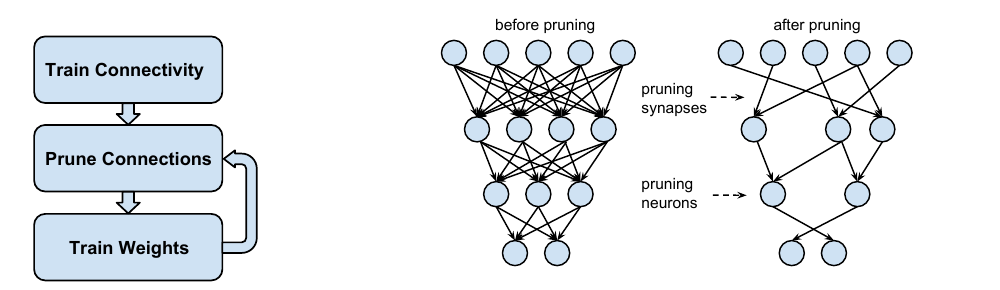
\includegraphics[width=0.78\textwidth,height=0.38\textheight,keepaspectratio]{images/inference-optimisation/han_pruning_pipeline_synapses_neurons.png}\\[0.15em]
  {\scriptsize Han et al., ``Learning both Weights and Connections for Efficient Neural Networks,'' \href{https://arxiv.org/abs/1506.02626}{arXiv:1506.02626}, Figures 2--3.}
\end{frame}

\begin{frame}{Pruning: Structure Matters}
  \begin{itemize}\itemsep0.5em
    \item[\textcolor{red}{$\blacktriangleright$}] \textbf{Unstructured pruning} removes individual weights: highest compression, but the result is a sparse matrix that standard GPU kernels cannot run faster.
    \item[\textcolor{red}{$\blacktriangleright$}] \textbf{Structured pruning} removes whole neurons, attention heads, or layers: less aggressive, but leaves a smaller dense model that is faster on any hardware.
    \item[\textcolor{red}{$\blacktriangleright$}] \textbf{2:4 semi-structured sparsity:} keep 2 weights in every group of 4; NVIDIA tensor cores (Ampere onward) run it at up to 2$\times$ math throughput (Mishra et al., 2021).
    \item[\textcolor{red}{$\blacktriangleright$}] For LLMs, one-shot post-training methods (SparseGPT, Wanda) reach about 50\% sparsity with modest quality loss and no retraining.
    \item[\textcolor{red}{$\blacktriangleright$}] Pruning composes with distillation and quantization; production LLM serving still leans mostly on quantization, with pruning gaining ground through 2:4 hardware support.
  \end{itemize}
\end{frame}
